\documentclass[12pt, a4paper]{report}
\usepackage{epsfig}
\usepackage{subfigure}
%\usepackage{amscd}
\usepackage{amssymb}
\usepackage{amsbsy}
\usepackage{amsmath}
\usepackage{amsthm}
\usepackage{framed}
\usepackage{subfiles}
%\usepackage[dvips]{graphicx}
\usepackage{natbib}
\bibliographystyle{chicago}
\usepackage{vmargin}
% left top textwidth textheight headheight
% headsep footheight footskip
\setmargins{3.0cm}{2.5cm}{15.5 cm}{22cm}{0.5cm}{0cm}{1cm}{1cm}
\renewcommand{\baselinestretch}{1.5}
\pagenumbering{arabic}
\theoremstyle{plain}
\newtheorem{theorem}{Theorem}[section]
\newtheorem{corollary}[theorem]{Corollary}
\newtheorem{ill}[theorem]{Example}
\newtheorem{lemma}[theorem]{Lemma}
\newtheorem{proposition}[theorem]{Proposition}
\newtheorem{conjecture}[theorem]{Conjecture}
\newtheorem{axiom}{Axiom}
\theoremstyle{definition}
\newtheorem{definition}{Definition}[section]
\newtheorem{notation}{Notation}
\theoremstyle{remark}
\newtheorem{remark}{Remark}[section]
\newtheorem{example}{Example}[section]
\renewcommand{\thenotation}{}
\renewcommand{\thetable}{\thesection.\arabic{table}}
\renewcommand{\thefigure}{\thesection.\arabic{figure}}
\title{Research notes: linear mixed effects models}
\author{ } \date{ }


\begin{document}
	\author{Kevin O'Brien}
	\title{Mixed Models for Method Comparison Studies}
	
	\addcontentsline{toc}{section}{Bibliography}
	
	
	
	
	%	
	%	\citet{schabenberger} describes the examination of model-data agreement as comprising several elements; \begin{itemize}
	%		\item residual analysis,
	%		\item goodness of fit,
	%		\item collinearity diagnostics
	%		\item influence analysis.
	%	\end{itemize}
	%	
	%\end{abstract}
	\chapter{Residual Analysis and Influence Diagnostics for Method Comparison}
	Model validation and model appraisal are vital parts of the modelling process, yet are too often overlooked.	Using a small handful of simple measures and methods, such as the AIC and $R^2$ measures, is insufficient to properly assess the usefulness of a fitted model. A full and comprehensive
	analysis that comprises residual analysis and influence analysis for testing model assumptions, should be carried out.  In classical linear models model diagnostics are now considered a required part of any statistical analysis, and the methods are commonly available in statistical packages and standard textbooks on applied regression. However it has been noted by several papers \citep{Christensen, schabenberger} that model diagnostics do not often accompany LME model analyses.

	\section{Residual Analysis}
	In classical linear models, model diagnostics techniques determine whether or not the distributional assumptions are satisfied, and to assess the influence of unusual observations, and have been become a required part of any statistical analysis. Well established methods are commonly available in statistical packages and standard textbooks on applied regression. However it has been noted by several papers that model diagnostics do not often accompany LME model analyses. A residual is simply the difference between an observed value and the corresponding fitted value, as predicted by the model. As with classical models, there are two key techniques: a residual plot and the normal probability plot. The rationale is that, if the model is properly fitted to the model, then the residuals would approximate the random errors that one should expect.
	that is to say, if the residuals behave randomly, with no discernible trend, the model has fitted the data well. If some sort of non-random trend is evident in the model, then the model can be considered to be poorly fitted. 
	


However, for LME models the matter of residual is more complex, both from a theoretical point of view and from the practical matter of implementing a comprehensive analysis using statistical software. \citet{schabenberger} discusses residuals for LME model, providing a useful summary of various techniques. Prominent in literature is the taxonomy of residuals for LME Models, distinguishing between condition residuals, marginal residuals and EBLUPS, including \citet{ HildenMinton, schabenberger, west, NobreSinger2007}. The underlying assumptions for LME models are similar to those of classical linear mdoels. 

Statistical software environments, such as the \texttt{R} Programming language, provides a suite of tests and graphical procedures for appraising a fitted linear model, with several of these procedures analysing the model residuals. Texts such as \citet{PB,west,Galecki} describe what can be implemented for LME residual analyses with statistical software, such as \texttt{R} and \texttt{SAS}.


In the context of Method Comparison, a residual analysis would be carried out just as any other LME model would, testing normality. As such there is little scope for adding additional insights, other than to say that
it is possible to create plots specific to each method. The figures on the next page depict the residual analysis for the Blood data. This can be used to indicate which methods disagree with the rest, but these would be a confirmation of something detected previously.

Analysis of the residuals could determine if the methods of measurement disagree systematically, or whether or not erroneous measurements associated with a subset of the cases are the cause of disagreement. 
The figure depicts residual plot for the Systolic Blood Pressure example. Points are labelled by subjects, with cases 67, 68 and 71 being among the prominent cases. Prominent cases warrant further investigation, but an analyst should procede to influence diagnostics beforehand.

\begin{figure}[h!]
			\centering
			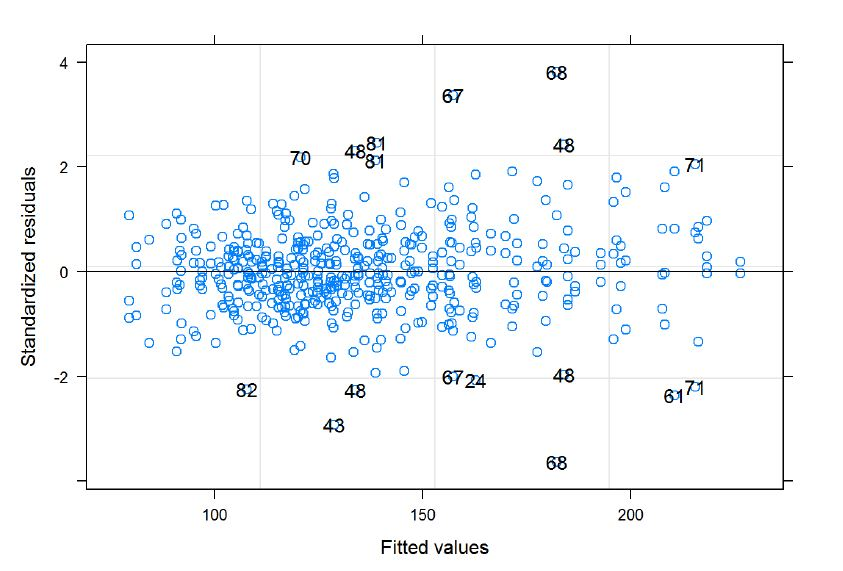
\includegraphics[width=0.8\linewidth]{images/Residuals-JS-Roy}
		\end{figure}
		
The next figure depicts residual plot for the Systolic Blood Pressure example, panelled by the various measurement methods. It serves to confirm agreement between methods J and R, with lack of agreement between those two methods and method S. However, little insight can be gained as to what actually causes lack of agreement here. 
\begin{figure}[h!]
\centering
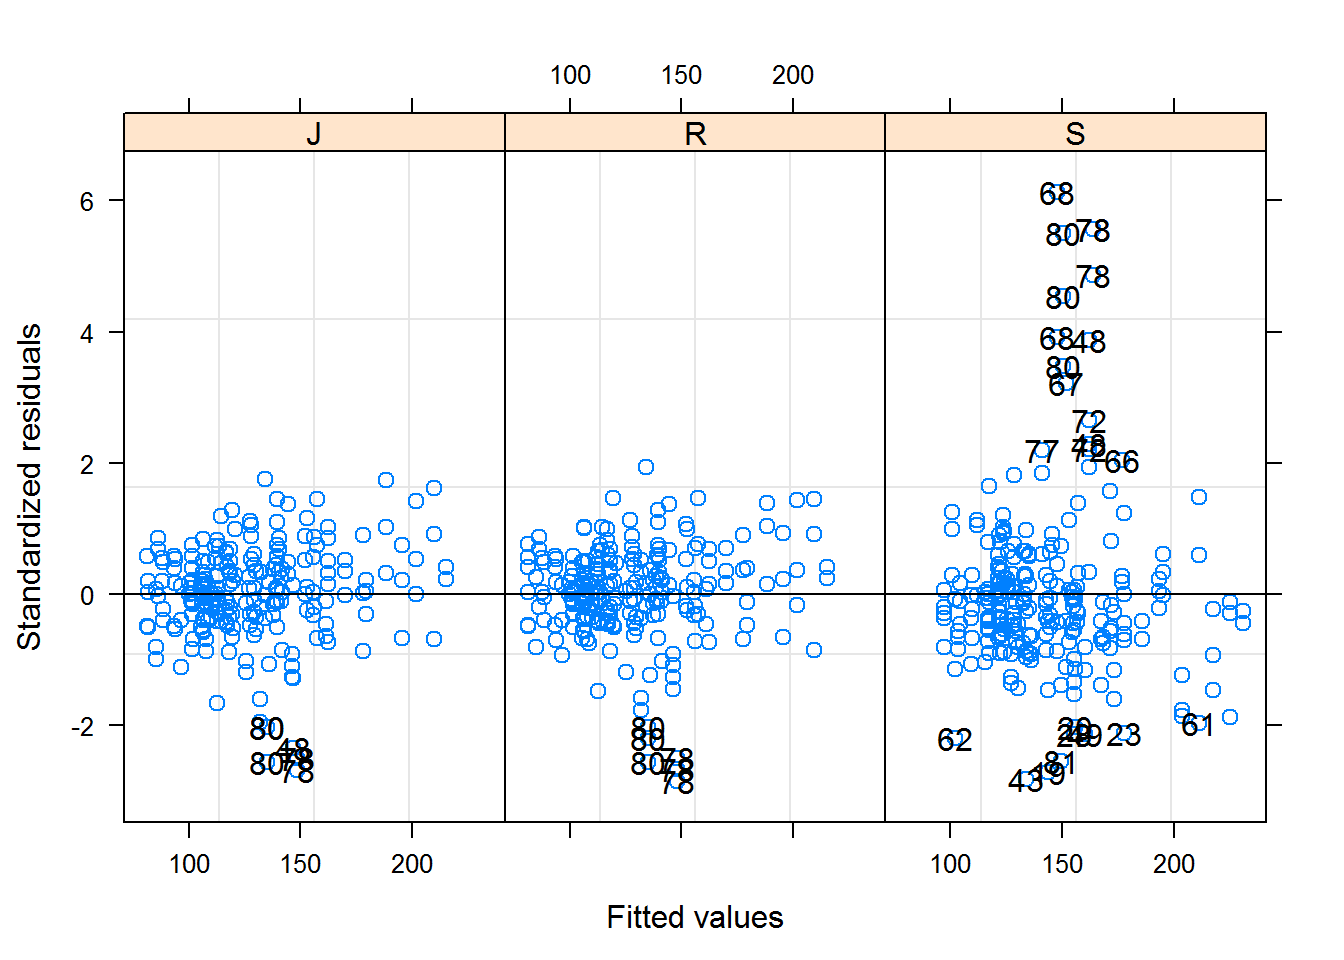
\includegraphics[width=0.8\linewidth]{images/bloodnlme-ResidPlot}
\caption{LME Residuals by Method (Blood Pressure Data)}

\end{figure}


\newpage			
	\section{Influence Diagnostics}

	Model diagnostic techniques can determine whether or not the distributional assumptions are satisfied, but also to assess the influence of unusual observations. 
	
	
	Following model specification and estimation, it is of interest to explore the model-data
	agreement by raising pertinent questions. Pinheiro and Bates provide some insight into how to compute and interpret model diagnostic plots for LME models. Unfortunately this aspect of LME theory is not as expansive as the corresponding body of work for Linear Models. Their particular observations will be reverted to shortly. Further to the analysis of residuals, \citet{schabenberger} recommends the examination of the following questions:
	\begin{itemize}
		\item Does the model-data agreement support the model assumptions?
		\item Should model components be refined, and if so, which components? For example, should certain explanatory variables
		be added or removed, and is the covariance of the observations properly specified?
		\item Are the results sensitive to model and/or data? Are individual data points or groups of cases particularly
		influential on the analysis?
	\end{itemize}
	
	The last of these three questions, regarding influential points, is of particular interest in the context of Method Comparison. After fitting an LME model, it is important to carry put model diagnostics to check whether distributional assumptions for the
	residuals as satisfied and whether the fit the model is sensitive to unusual assumptions. The process of carrying out model
	diagnostic involves several informal and formal techniques, which will mentioned throughout the chapter.

Influential points have a large influence on the fit of the model. Influential points are a set of one or more observations whose removal would cause a different conclusion in the analysis, e.g. substantially changes the estimate of the regression coefficients. \citet{west} remarks that influence diagnostics play an important role in the interpretation of results, because influential data can negatively 
	influence the statistical model and generalizability of the model.
	\citet{schabenberger} remarks that the concept of critiquing the model-data agreement applies in mixed models in the same way as in linear
	fixed-effects models. In fact, because of the more complex model structure, you can argue that model and
	data diagnostics are even more important \citep{west}.
	%Influential points have a large influence on the fit of the model. 
	
	%One approach for determining influential points is to compare the fit of the model with and without each observation.
	
	%The basic rationale behind identifying influential data is that when iteratively single units are omitted from the data, models based on these data should not produce substantially different estimates. 
		\subsection{A Procedure for Quantifying Influence}  
		
		\citet{schabenberger} describes a simple procedure for quantifying influence for LME Models. Firstly a model should be fitted to the data, and
		estimates of the parameters should be obtained. The second step is that either single or multiple data points, specifically outliers,
		should be omitted from the analysis, with the original parameter estimates being updated. This is known as \textit{leave one out} or \textit{leave k out} analysis. The final step of the procedure is comparing the sets of estimates computed from the entire and reduced data sets to determine whether the absence of observations changed the
		analysis. 

	
	%http://support.sas.com/documentation/cdl/en/statug/63033/HTML/default/viewer.htm#statug_mixed_sect024.htm
	
%\subsubsection{Outliers and Leverage}
	Influence can be thought of as consequence of leverage and outlierness. Outliers are the most noteworthy data points in an analysis, and an objective of influence analysis is how influential they are, and the manner in which they are influential. They can point to a model breakdown and lead to development of a better model.
	The linear mixed effects model is a useful methodology for fitting a wide range of models. However, linear mixed effects models are known to be sensitive to outliers. Specifically likelihood based estimation techniques, such as ML and REML, are sensitive to outliers. \citet{Christensen} advises that identification of outliers is necessary before conclusions may be drawn from the fitted model. The leverage of an observation is a further consideration. 
	
%The question of whether or not a point should be considered an outlier must therefore be addressed. An outlier is an observation whose true value is unusual given its value on the predictor variables.

An observation with an extreme, but not unusual, value on a predictor variable is a point with high leverage. High leverage points can have a great amount of effect on the estimate of regression coefficients. In general. a high leverage point means a extreme value for the one or more of the independent variables, and a greater potential of overly influencing the final fitted model. However, if a case has  extreme values for the independent variables but is fitted very well by a regression model, this case is not necessarily overly influential.

In classical linear models, leverages are the diagonal elements $h_{ii}$ of the Projection matrix, also known as the Hat Matrix $\boldsymbol{H}$. \citet{schabenberger} describes two analogues of $\boldsymbol{H}$ for LME models. However the practical use for either approach is not made clear.


	% - Leverage is a measure of how far an independent variable deviates from its mean.
	

%\subsection{Cook's 1986 paper on Local Influence}%1.7.1

\subsection{Analyzing Influence in LME models}

Model diagnostic techniques, well established for classical models, have since been adapted for use with linear mixed effects models. Diagnostic techniques for LME models are inevitably more difficult to implement, due to the increased complexity.

Influence diagnostics are formal techniques allowing for the identification of observations that exert substantial  influence on the estimates of fixed effects and variance covariance parameters.
While linear models and GLMS can be studied with a wide range of well-established diagnostic technqiues, the choice of methodology is much more restricted for the case of LMEs. However
	influence diagnostics for LME Models is an area of active research. Research on diagnostic analyses for LME models are presented in \citet{Beckman}, 
	\citet{Christensen}, \citet{HildenMinton}, \citet{lesaffre1998local}, \citet{Banerjee1997}, 
	\citet{fung2002}, \citet{Demi}, \citet{Zewotir}, \citet{zewotir2008} and \citet{NobreSinger2007, NobreSinger2011}.
	
	
	
	
	
	\citet{schabenberger} states that goal of influence analysis is not primarily to mark data
	points for deletion so that a better model fit can be achieved for the reduced data, although this might be a
	result of influence analysis. The goal is rather to determine which cases are influential and the manner in
	which they are important to the analysis. 



%For example, you are not only concerned with capturing the fixed and random components of the model. The LME model structure presents unique and interesting challenges that prompt us to reexamine the traditional ideas of influence and residual analysis.
%








%============================================================================================== %
%Influence arises at two stages of the LME model. Firstly when $V$ is estimated by $\hat{V}$, and subsequent
%estimations of the fixed and random regression coefficients $\beta$ and $u$, given $\hat{V}$.
%
%Diagnostic methods for fixed effects are generally analogues of methods used in classical linear models.
%Diagnostic methods for variance components are based on `one-step' methods. 

%======================================================= %
\subsection{Measuring of Influence for LME Models}
%- (Zewotir) 
Influence analysis methodologies have been used extensively in classical linear models, and provided the basis for methodologies for use with LME models. Computationally inexpensive diagnostics tools have been developed to examine the issue of influence \citep{Zewotir}. 


\citet{Zewotir} remarks the development of efficient computational formulas is crucial making deletion diagnostics useable, allowing one to obtain the \index{case deletion diagnostics} case deletion diagnostics by making use of basic building blocks, computed only once for the full model. A number of approaches to model diagnostics are described, including variance components, dixed effects parameters, prediction of the response variable and of random effects, and the likelihood function. Influence statistics can be grouped by the aspect of estimation that is their primary target:
\begin{itemize}
	\item \textbf{overall measures compare changes in objective functions}: (restricted) likelihood distance (Cook and Weisberg 1982, Ch. 5.2)
	\item \textbf{influence on parameter estimates}: Cook's  (Cook 1977, 1979), MDFFITS (Belsley, Kuh, and Welsch 1980, p. 32)
	\item \textbf{influence on precision of estimates}: CovRatio and CovTrace
	\item \textbf{influence on fitted and predicted values}: PRESS residual, PRESS statistic (Allen 1974), DFFITS (Belsley, Kuh, and Welsch 1980, p. 15)
	\item \textbf{outlier properties}: internally and externally studentized residuals, leverage
\end{itemize}


\citet{Zewotir} lists several established methods of analyzing influence in LME models. These methods include Cook's distance for LME models,
\index{likelihood distance} likelihood distance,
the variance (information) ration,
the \index{Cook-Weisberg statistic} Cook-Weisberg statistic, and
the \index{Andrews-Prebigon statistic} Andrews-Prebigon statistic.

The subscript $(U)$ is used to denote quantities computed from data with subset of cases $U$ omitted.
If the global measure suggests that the points in $U$ are influential, you should next determine the nature of
that influence. In particular, the points can affect
\begin{itemize}
	\item the estimates of fixed effects
	\item the estimates of the precision of the fixed effects
	\item the estimates of the covariance parameters
	\item the estimates of the precision of the covariance parameters
	\item fitted and predicted values
\end{itemize}	

For example, if observations primarily affect the precision of the covariance parameters without exerting much influence on the fixed effects, then their presence in the data may not distort hypothesis
tests or confidence intervals about $\beta$. 
\citet{schabenberger} notes that removing observations or sets of observations affects fixed effects and covariance parameter estimates.





\subsection{Deletion Diagnostics}

%Data from single individuals, or a small group of subjects may influence non-linear mixed effects model selection. 
%Diagnostics routinely applied in model building may identify such individuals, but these methods are not specifically designed for that purpose and are, therefore, not optimal. 
%We describe two likelihood-based diagnostics for identifying individuals that can influence the choice between two competing models.


Deletion diagnostics provide a means of assessing the influence of an observation (or groups of observations) on parameters inferences for a fitted model. For classical linear models, \citet{cook77} greatly expands the study of residuals and influence measures. The key to making deletion diagnostics useable is the development of efficient computational formulas, allowing one to obtain the \index{case deletion diagnostics} case deletion diagnostics by making use of basic building blocks, computed only once for the full model.
Cook's key observation was the effects of deleting each observation in turn could be calculated with little additional computation. Cook proposed a measure that combines the information of leverage and residual of the observation, now known simply as the Cook's Distance, $D_{(i)}$, which can be calculated without fitting a new regression coefficient each time an observation is deleted. Consequently deletion diagnostics have become an integral part of assessing linear models.



It must be pointed out that the effect on the precision of estimates is separate from the effect on the point estimates. Data points that have a small \index{Cook's distance}Cook's distance, for example, can still greatly affect hypothesis tests and confidence intervals, if their 
influence on the precision of the estimates is large.	

\citet{Christensen} notes the case deletion diagnostics techniques have not been applied to linear mixed effects models and seeks to develop methodologies in that respect. \citet{Christensen} developed their global influences for the deletion of single observations in two steps: a one-step estimate for the REML (or ML) estimate of the variance components, and an ordinary case-deletion diagnostic for a weighted resgression problem (conditional on the estimated covariance matrix) for fixed effects.

The computation of case deletion diagnostics in the classical model is made simple by the fact that estimates of $\beta$ and $\sigma^2$, which exclude the $i$th observation, can be computed without re-fitting the model. Such update formulas are available in the mixed model only if you assume that the covariance parameters are not affected by the removal of the observation in question. This is rarely a reasonable assumption, and undermines the use of many proposed procedures for Method Comparison.

	\subsection{Cook's Distance}
As previously described, \index{Cook's Distance} Cooks Distance ($D_{i}$) is a diagnostic technique used in classical linear models, that functions as an overall measure of the influence of an observation that is a measure of aggregate impact of each observation on the group of regression coefficients, as well as the group of fitted values. \index{Cook's distance} Cook's Distance as a measure of the influence of observations in subset $U$ on a vector of parameter estimates is given below \citep{cook77}
	\[ \delta_{(U)} = \hat{\beta} - \hat{\beta}_{(U)}.\]
	Observations, or sets of observations, that have high Cook's distance usually have high residuals, although this is not necessarily the case.
	
	
	%Cook's Distance is proportional to the sum of the squared differences between predictions made with all observations in the analysis and predictions made leaving out the observation in question.
	If the predictions are the same with or without the observation in question, then the observation has no influence on the regression model. If the predictions differ greatly when the observation is not included in the analysis, then the observation is influential.
	
	%======================================================================================= %
	

	Large values for Cook's distance indicate observations for special attention. Cook's distance can be used in several ways: to indicate data points that are particularly worth checking for validity; to indicate regions of the design space where it would be good to be able to obtain more data points.
	
	
	
	Use of threshold values for Cook's Distance is discouraged \citep{fox1997}. However, informal heuristics do exist for OLS models; Obervations for which Cook's distance is higher than 1 are usually considered as influential. Another informal threshold of $4/n$ or $4/(n-k-1)$, where $n$ is the number of observations and $k$ the number of explanatory variables.
	\citet{fox1997} advises the use of diagnostic plotting and to examine in closer details the points with \textit{``values of D that are substantially larger than the rest}", and that thresholds should feature only to enhance graphical displays.
	
	
	The effect on the precision of estimates is separate from the effect on the point estimates. Data points that have a small \index{Cook's distance}Cook's distance, for example, can still greatly affect hypothesis tests and confidence intervals, if their  influence on the precision of the estimates is large.
	

	\citet{Christensen} develops \index{case deletion diagnostics} case deletion diagnostics, in particular the equivalent of \index{Cook's distance} Cook's distance for diagnosing influential observations when estimating the fixed effect parameters and variance components, adapting the \index{Cook's distance}Cook's Distance measure for the analysis of LME models. For LME models, two formulations exist; a \index{Cook's distance}Cook's distance that examines the change in fixed fixed parameter estimates, and another that examines the change in random effects parameter estimates. The outcome of either Cook's distance is a scaled change in either $\beta$ or $\theta$. \citet{Zewotir} gives a detailed discussion of the various formulation for Cook's distances for LME Models.

\begin{figure}[h!]
	\centering
	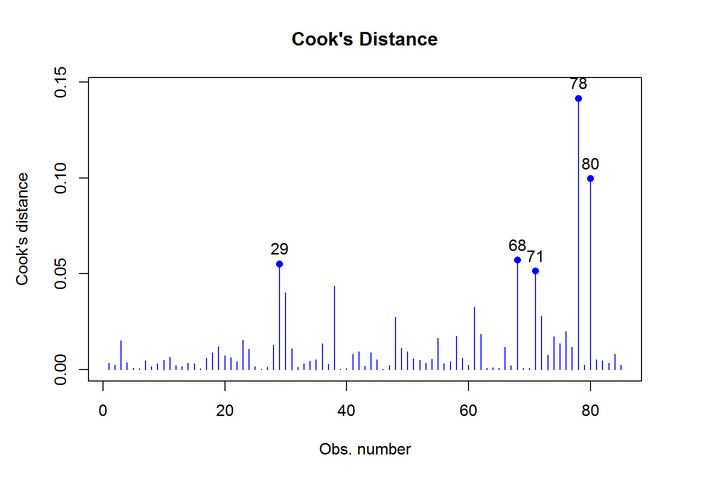
\includegraphics[width=0.7\linewidth]{images/CooksDistancePlot-JS-Roy}
	\caption{}
	\label{fig:CooksDistancePlot-JS-Roy}
\end{figure}	
	%	For LME models, Cook's distance can be extended to model influence diagnostics by defining:
	%	\[ C_{\beta i} = {(\hat{\beta} - \hat{\beta}_{[i]})^{T}(\boldsymbol{X}^{\prime}\boldsymbol{V}^{-1}\boldsymbol{X}) (\hat{\beta} - \hat{\beta}_{[i]}) \over p}\]
	%	
	%	It is also desirable to measure the influence of the case deletions on the covariance matrix of $\hat{\beta}$.
	
	%	It uses the same structure for measuring the combined impact of the differences in the estimated regression coefficients when the $i$th case is deleted. Importantly, $D_{(i)}$ can be calculated without fitting a new regression coefficient each time an observation is deleted.
	
	%Cook's Distance is proportional to the sum of the squared differences between predictions made with all observations in the analysis and predictions made leaving out the observation in question.

	
	
	
%
%	
%	If V is known, Cook's D can be calibrated according to a chi-square distribution with degrees of freedom equal to the rank of $\boldsymbol{X}$ \citep{cpj92}.
%	
%	
	










%		
%		
%		In this section we introduce influence analysis and case deletion diagnostics. A full overview of the topic will be provided although there are specific tools that are particularly useful in the case of Method Comparison problems: specifically the Cook's Distance and the DFBETA.




Consideration of how leave-$U$-out diagnostics would work in the context of Method Comparison problems is required. There are several scenarios. \citet{preisser} describes two type of diagnostics. When the set consists of only one observation, the type is called
`\textit{observation-diagnostics}'. For multiple observations, Preisser describes the diagnostics as `\textit{cluster-deletion}' diagnostics. Suppose we have two methods of measurement X and Y, each with three measurements for a specific case: $(x_1,x_2,x_3,y_1,y_2,y_3)$

\begin{itemize}
	\item Leave One Out - one observation is omitted (e.g. $x_1$)
	\item Leave Pair Out - one pair of observation  is omitted (e.g. $x_1$ and $y_1$)
	\item Leave Case (or Item or Subject) Out - All observations associated with a particular case or subject are omitted. (e.g. $\{x_1,x_2,x_3,y_1,y_2,y_3\}$)
\end{itemize}
%% Schabenberger
%%

The natural sampling unit is the item or subject, similar to the example provided by \citet{schabenberger}. Hence, the third option, henceforth, referred to as ``Leave subject Out" will be the option used.


\subsection{Local Influence}
\citet{cook86} gives a completely general method for assessing the influence of local departures from assumptions in statistical models, introducing methods for local influence assessment for classical linear models. These methods provide a powerful tool for examining perturbations in the assumption of a model, particularly the effects of local perturbations of parameters of observations. The local-influence approach to influence assessment is quite different from the case deletion approach, comparisons are of interest.

% % Beckman, Nachtsheim and Cook (1987)
\citet{Beckman} applied the \index{local influence}local influence method of Cook (1986) to the analysis of the LME model.  Other authors such as \citet{lesaffre1998local} have also extended these idea to LME models. 
While the concept of influence analysis is straightforward, implementation in mixed models is more complex. Update formulae for fixed effects models are available only when the covariance parameters are assumed to be known. As such the local influence approach are not particularly useful in the context of Method Comparison, and so will not be considered further.





\subsection{Comparing Influence and Residual Analysis}
%In LME models, there are two types of residuals, marginal residuals and conditional residuals. A
%marginal residual is the difference between the observed data and the estimated marginal mean. A conditional residual is the
%difference between the observed data and the predicted value of the observation. In a model without random effects, both sets of residuals coincide \citep{schab}.

\citet{influenceLME4} compares residual analysis and influence analysis. Cases with high residuals (defined as the difference between the observed and the predicted scores on the dependent
variable) or with high standardized residuals (defined as the residual divided by the standard deviation
of the residuals) are indicated as outliers.

However, an influential case is not necessarily an outlying residual. On the contrary: a strongly influential case dominates
the regression model in such a way, that the estimated regression line lies closely to this case. The analysis of residuals cannot be used for the detection of influential cases \citep{crawley2012r}.



	


%\subsection{Extension of Diagnostic Methods to LME models}

 




%============================================================================================================================ %


\subsection{Iterative and Non-Iterative Influence Analysis}




%----schabenberger page 8
For linear models, the implementation of influence analysis is straightforward, but for LME models the process is more complex. \citet{schabenberger} examines the use and implementation of
influence measures in LME models. \citet{schabenberger} highlights some of the issue regarding implementing LME model diagnostics, describing  the choice between \index{iterative influence analysis} iterative influence analysis and \index{non-iterative influence analysis} non-iterative influence analysis.
\citet{schabenberger} considers several important aspects of the use and implementation of influence measures in LME models, noting that it is not always possible to
derive influence statistics necessary for comparing full- and reduced-data parameter estimates. Closed-form expressions for computing the change in important model quantities might not be available.

On a related matter, \citet{schabenberger} describes the scenario wherein a data point is removed and the new estimate of the $D$ matrix is not positive definite. This may occur if a variance component
estimate now falls on the boundary of the parameter space \citep{schabenberger}. 

%%Non-Iterative
For classical linear models, it is not necessary to refit the model after removing a data point in order to measure the impact of an observation on the model. The change in fixed effect estimates, residuals, residual sums of squares, and the variance-covariance matrix of the fixed effects can be computed based on the fit to the full data alone, using update formulas \citep{sherman, hager1989}.



However, in LME models several important complications arise. Data points can affect not only the fixed effects but also the covariance parameter estimates on which the fixed-effects estimates depend.

When applied to LME models, such update formulas are available only if one assumes that the covariance parameters are not affected by the removal of the observation in question. However, this is rarely a reasonable assumption.
For LME models, non-iterative methods are computationally efficient, but require the rather strong assumption that all 
covariance parameters are known, and thus are not updated, with the exception of the profiled residual variance.
Update formulas for ``leave-U-out" estimates typically fail to account for changes in covariance parameters.  As the influence that each item would have on the variance estimate of a method comparison model is crucial, this substanitally negates their usefulness for Roy's Model.

%============================================%
%%Iterative
Iterative influence diagnostics requiring fitting the model without the observations in question. Computation execution time is substantially longer, although this is balanced by algorithmic 
simplicity, with no assumptions beyond those used for the original model. A measure of total influence requires updates of all model parameters. This can only be achieved in general is by omitting observations or cases, then refitting the model. 


An iterative analysis may seem computationally expensive. Computing iterative influence diagnostics for $n$ observations
requires $n+1$ mixed models to be fitted iteratively.
The execution times for iterative procedures are longer relative to non-iterative procedures, but are not so long that they would dissuade an analyst from using them.
Despite the addition execution time of iteratives
approaches, they are preferable for Method Comparison problems, as they can facilitate several complementary analyses concurrently. 


Iterative methods retain the potential for useful analyses, if applied at different stage of the modelling process. Diagnostic measures, specifically the DFBETA, have characteristics that would make them very useful at the exploratory stage of the method comparison process. Implicitly various assumptions about variance are used, but simultaneously an approach based on DFBETA can be used to assess if these assumptions are valid.



\subsection{Likelihood Distance}
An overall influence statistic measures the change in the objective function being minimized. For example, in
classical linear, the residual sums of squares serves that purpose. In linear mixed models fit by
\index{maximum likelihood} maximum likelihood (ML) or \index{restricted maximum likelihood} restricted maximum likelihood (REML), an overall influence measure is the \index{likelihood distance} likelihood distance \citep{CookWeisberg}.

%	\subsection{Likelihood Distances}

The \index{likelihood distance} likelihood distance is a global summary measure that expresses the joint influence of the subsets of observations, $U$, on all parameters that were subject to updating. \citet{schabenberger} points out that the likelihood distance $LD(\psi_{(U)})$ is not the log-likelihood obtained by fitting the model to the reduced data set. Instead it is obtained by evaluating the likelihood function based on the full data set (containing all $n$ observations) at the reduced-data estimates.




%==========================================================%
%	\subsubsection{Likelihood Distances}

 The
procedure requires the calculation of the full data estimates
$\hat{\psi}$ and estimates based on the reduced data set
$\hat{\psi}_{(U)}$. The likelihood distance is given by
determining
\[
LD_{(U)} = 2\{l(\hat{\psi}) - l( \hat{\psi}_{(U)}) \}\]\[
RLD_{(U)} = 2\{l_{R}(\hat{\psi}) - l_{R}(\hat{\psi}_{(U)})\}
\]
Large values indicate that $\boldsymbol{\hat{\theta}}$ and $\boldsymbol{\hat{\theta}_\omega}$ differ considerably.

\citet{west} examines a group of methods that examine various aspects of influence diagnostics for LME models. For overall influence, the most common approaches are the \textit{likelihood distance} and the \textit{restricted likelihood distance}.

%For noniterative methods the following computational devices are used to compute (restricted) likelihood distances provided that the residual variance
%$\sigma^2$ is profiled.


\section{Model Diagnostics for Roy's Models}

Further to previous work, this section revisits case-deletion and residual diagnostics, and explores how approaches devised by  \citet{Galecki} can be used to appraise Roy's model. These authors specifically look at Cook's Distances and Likelihood Distances.
%	For the Roy Model, Cook's Distances may also be generated using the \textbf{\textit{predictmeans}}
%	





\begin{figure}[h!]
	\centering
	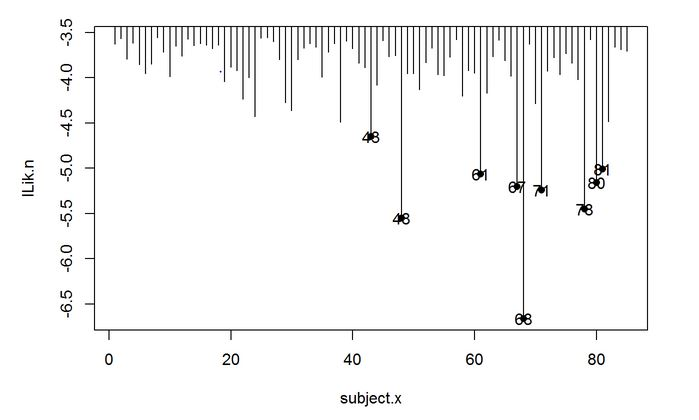
\includegraphics[width=0.7\linewidth]{images/LogLik-JS-Roy}
	\caption{}
	\label{fig:LogLik-JS-Roy}
\end{figure}








\subsubsection{Case Deletion Diagnostics for Variance Ratios}


Taking the core principals of his methods, and applying them to the Method Comparison problem, case deletion diagnostics are used on the variance components of the Roy's model, specifically the ratio of between subject variances and the within subject covariances respecitvely.


\[ \mbox{BSVR} = \frac{\sigma^2_2}{\sigma^2_2} \phantom{makespace}  \mbox{WSVR} = \frac{d^2_2}{d^2_2} \]

These variance ratios are re-computed for each case removed, and may be analysed seperately or jointly for outliers.




%\subsubsection{Methods for Identifying Outliers}
The Grubbs' Test for Outliers is a commonly used technique for assessing outlier in a univariate data set, of which there are several variants.
As there may be several outliers present, the Grubbs test is not practical. However an indication that a point being beyond the fences according to Tukey's specification for boxplots will suffice.


% The first variant of Grubb's test is used to detect if the sample dataset contains one outlier, statistically different than
% the other values. The test statistic is based by calculating score of this outlier $G$ (outlier minus mean and divided
% by the standard deviation) and comparing it to appropriate critical values. Alternative method is calculating ratio of
% variances of two datasets - full dataset and dataset without outlier.
% %The obtained value called U is bound with G by simple formula.
% The second variant is used to check if lowest and highest value are two outliers on opposite tails of sample. It is based on calculation of ratio of range to standard deviation of the sample.
% 
% The third variant calculates ratio of variance of full sample and sample without two extreme observations.
% It is used to detect if dataset contains two outliers on the same tail.



The WSVR values are plotted against the corresponding BSVR values, with commonly used bivariate methods may be applied jointly to the both sets of data sets, e.g Mahalanobis distances. Confidence ellipses can be superimposed over the plot with minimal effort. Two ellipses are generated by this technique, a 50 \% and 97.5\% confidence ellipse respectively. Outlying cases are idenified by the plot. Subject 68 is the most prominent case.

The subjects were ranked by Mahalanobis distance, with the top 10 being presented in the following table. Both sets of ratio are addtionally expressed as a ratio of the full model variance ratios.
\begin{center}
	\begin{tabular}{|c|c|c|c|c|c|}
		\hline
		Subject (u) &  MD & WSVR$_{(u)}$ & WSVR (\%) & BSVR$_{(u)}$   & BSVR (\%)     \\ \hline \hline
		68 & 44.7284   & 1.3615  & 0.9132   & 1.0353  & 0.9849 \\ \hline
		30 & 16.7228   & 1.5045  & 1.0092   & 1.1024  & 1.0487 \\ \hline
		71 & 11.5887   & 1.5210  & 1.0202   & 1.0932  & 1.0400 \\ \hline
		80 & 11.0326   & 1.4796  & 0.9925   & 1.0114  & 0.9621 \\ \hline
		38 & 10.3671   & 1.5011  & 1.0069   & 1.0917  & 1.0385 \\ \hline
		67 & 10.1940   & 1.4308  & 0.9598   & 1.0514  & 1.0002 \\ \hline
		43  & 7.6932   & 1.4385  & 0.9649   & 1.0511  & 0.9999 \\ \hline
		72  & 4.7350   & 1.4900  & 0.9995   & 1.0262  & 0.9762 \\ \hline
		48  & 4.4321   & 1.4950  & 1.0028   & 1.0280  & 0.9779 \\ \hline
		29  & 4.3005   & 1.4910  & 1.0001   & 1.0769  & 1.0244 \\ \hline
	\end{tabular}
\end{center}
From this table one may conclude that subjects 72, 48 and 29 are not particularly influential. Interestingly Subject 78, which was noticeable in the case deletion diagnostics for fixed effects, does not feature in this table.

\begin{figure}[h!]
	\centering
	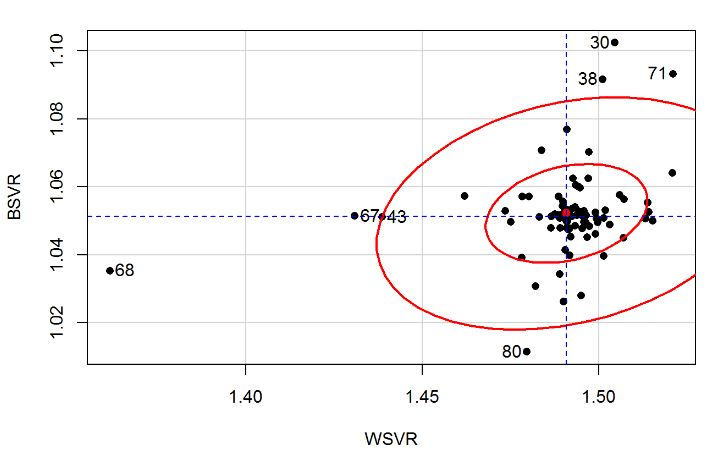
\includegraphics[width=0.9\linewidth]{08-plot1}
	\caption{}
	\label{fig:08-plot1}
\end{figure}



%===========================================================================%

\subsubsection{Variance Ratios}

The relationship between precision and the within-item and between-item variability must be established. Roy establishes the equivalence of repeatability and within-item variability, and hence precision.  The method with the smaller within-item variability can be deemed to be the more precise.

A useful approach is to compute the confidence intervals for the ratio of within-item standard deviations (equivalent to the ratio of repeatability coefficients), which can be interpreted in the usual manner.
%	

Pinheiro and Bates (pg 93-95) give a description of how confidence intervals for the variance components are computed. Furthermore a complete set of confidence intervals can be computed to complement the variance component estimates.

What is required is the computation of the variance ratios of within-item and between-item standard deviations.

A naive approach would be to compute the variance ratios by relevant F distribution quantiles. However, the question arises as to the appropriate degrees of freedom.
Bootstrap methods for computing confidence intervals may be considered.







\section{Using DFBETAs from LME Models to Assess Agreement}

	The impact of an observation on a regression fitting can be determined by the difference between the estimated regression coefficient of a model with all observations and the estimated coefficient when the particular observation is deleted. DFBETA and DFFITS are well known measures of influence. Emphasis shall be placed on DFBETA, but a brief discussion of DFFITS is merited as it potentially provides for useful techniques in method comparison. \citet{schabenberger} provides a mathematical desciption of both.
	
	 DFBETAS is a standardized measure of the absolute difference between the estimate with a particular
	case included and the estimate without that particular case,, thus measuring the impact each observation has on a particular predictor \citep{belsley2005}. For LME models, the DFBETA is a measure that standardizes the absolute difference in parameter estimates between an LME model based on a full set of data, and a model from reduced data.


 
	
In general, large values of DFBETAS indicate observations that are influential in estimating a given parameter. \citet{belsley2005} recommend 2 as a general cutoff value to indicate influential observations and as a size-adjusted cutoff. There is no agreement as to the critical threshold for DFBETAs. The cut-off value for DFBETAs is $\frac{2}{\sqrt{n}}$, where $n$ is the number of observations. However, another cut-off is to look for observations with a value greater than 1.00. Here cutoff means,
``this observation could be overly influential on the estimated coefficient".

 DFFITS is a diagnostic meant to show how influential a point is in a statistical regression. It is defined as the change, in the predicted value for a point, obtained when that point is left out of the regression, divided by the estimated standard deviation of the fit at that point:


	

	

	\subsubsection{DFBETAs for Method Comparison}
	
	For LME models, a value for DFBETAS is calculated for each of the $k$ fixed effects, and for each of the $n$ item. Correctly there will be $p+1$ DFBETAs (the intercept, $\beta_0$, and one $\beta$ for each covariate). When the LME model is specified without an intercept term, as in Roy's Model, there is a set of DFBETAs corresponding to each measurement method, hence an $n \times p$ matrix.
	
	In the case of method comparison studies, a series of scatterplots can be constructed to compare each pair of measurement methods.
	Furthermore 95\% confidence ellipse can be constructed around these scatterplots.
	
	
	
	The LME approach proposed by \citet{ARoy2009} is constrained by computational tractability.
	Consequently a simpler LME formulation is used, one similar to that of \citet{BXC2008}. However one constraint that can be dispensed with is the restriction to
	two methods of measurement: we can now use any number of methods.
	The benefit of using this model is that metrics such as Cook's Distance and DFBETAs can be computed also.

Furthermore, these measures form the basis of the analysis, rather than the estimates derived from the model. In the context of method comparison, these variables are the methods of measurement.
Agreement will considered in the context of inter-method bias and the within-item variance ratio. Between-item variance ratio is not considered for this analysis.

For a Method Comparison study, DFBETAs can be used as a proxy measurement, allowing simple techniques to be used for assessing agreement. Suppose an LME model was formulated to model agreement for two or more methods of measurement, specifically with replicate measurements. If the methods are to be agreement, the DFBETAs for each case would be the same for both methods. As such, agreement between any two methods can be determined by a simple scatterplot of the DFBetas. 
	

If the lack of agreement is caused, in part or in full, by differing within-item variances, there would be differing DFBETAs for each pair of methods. If the points align along the line of equality, then both methods can be said to be in agreement for within item variance. However DFBETAs are not useful for determining inter-method bias. If there is good agreement between methods, or if lack of agreement is caused by inter-method bias only, the DFBETA values will be almost identical for each subject in the data set. 
	
Following the idea proposed by \citet{BA86}, an identity plot to visually inspect this relationship between sets of DFBETAs. Modern statistical software usually allows for the creation of co-plots, so a grid of identity plots may be easily rendered for comparing each pair of methods. Used in conjection with a Bland-Altman plot, this co-plot can quickly determine agreement and indicate the source of lack of agreement.

For an LME model fitted to the Blood data, the results tabulated below can be produced.  Cases can be ranked by the Cook's Distance, such that the most divergent DFBETA are highlighted, with the top 6 being presented below). The remaining columns are the DFBeta for each of the fixed effects, for each of the 85 subject.
	\begin{center}
		\begin{tabular}{|c|c|c|c|c|} \hline
			Subject &    Cook's D  &    Method J  &   Method R  & Method S \\ \hline \hline
			78 & 0.61557407 & -0.02934556 & -0.03387780 & 0.2954937  \\ \hline
			80 & 0.41590973 & -0.06305026 & -0.06515241 & 0.2123881  \\ \hline
			68 & 0.22536651 & -0.05334867 & -0.05062375 & 0.1555187  \\ \hline
			72 & 0.09348500  & 0.02388626  & 0.02419887 & 0.1617474  \\ \hline
			48 & 0.08706988  & 0.02147541  & 0.03145273 & 0.1581591  \\ \hline
			30 & 0.07118415  & 0.26925807  & 0.26215970 & 0.1581569  \\ \hline
		\end{tabular}
	\end{center}
For DFBETA identity plots are presented below. This set of plots indicate agreement between methods J and R in terms of within-item variance, while severe lack of agreement exists between these methods and the third method S, as is the conclusion of \citet{ARoy2009}.	
	\begin{figure}[h!]
		\centering
		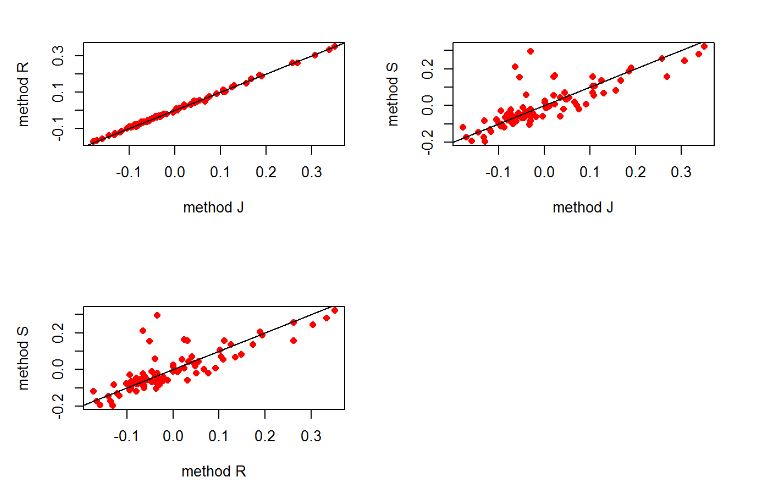
\includegraphics[width=1\linewidth]{images/04-DFbetaplots}
		% \caption{}
		% \label{fig:04-DFbetaplots}
	\end{figure}
	
If lack of agreement is indicated, a subsequent analysis using a technique proposed by \citet{ARoy2009} can be used to identify the specific cause for this lack of agreement.
	
Other analyses may be used to complement these plots. The Pearson Correlation coefficient of the DFBETAs can be used in conjection with this analysis. A high correlation confirms good agreement, thouhg no threshold value for agreement is suggested.
	
The Bonferroni Outlier Test and Cook's Distance values can be used to identify unusual cases, when the relationship between sets of DFBETA is modelled as a (classical) linear model. In this model, the covariates should be homoskedastic. A test for non-constant variance may be used to verify this. 
	
	
As an alternative to scatterplots, a mean difference plot could be used to assess agreement of with-item variance. This mean-difference plot differs from the Bland-Altman plot in that the plot is denominated in terms of DFBETA values, and not in measurement units. Here two of the three pairs of methods are compared on the same plot, red points indicate the J-R comparison while blue points are for the J-S comparison.

	\begin{figure}[h!
		]
		\centering
		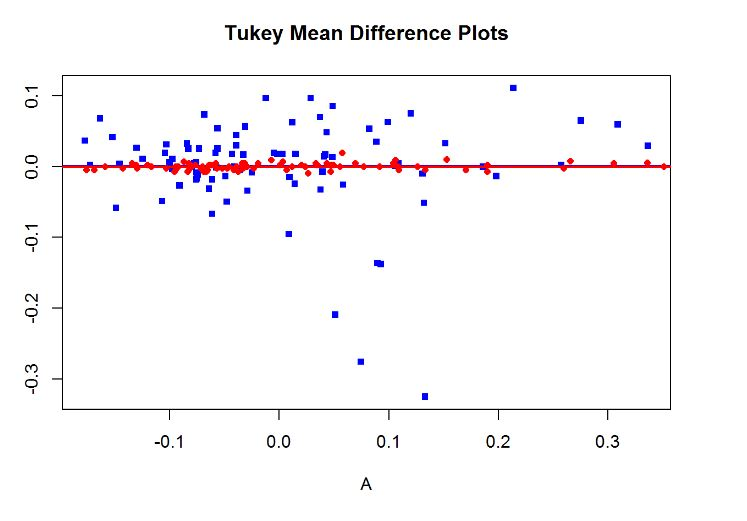
\includegraphics[width=0.7\linewidth]{images/04-TMDplot}
		
	\end{figure}
	
%============================================== %
%- F:
\bibliographystyle{chicago}
\bibliography{DB-txfrbib}

\end{document}


